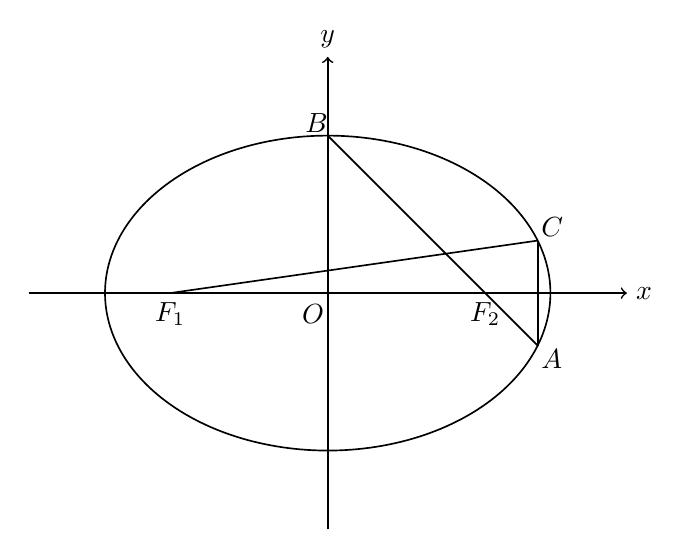
\begin{tikzpicture}[x=2cm,y=2cm,line width=.6pt]
\tikzset{lbl/.style={font=\normalsize,inner sep=1pt,fill=none}}
% ellipse x^2/2+y^2=1
\draw[domain=0:360,samples=220,variable=\t] plot ({1.41421356*cos(\t)},{sin(\t)});
% axes
\draw[->] (-1.9,0) -- (1.9,0) node[lbl,right=2pt] {$x$};
\draw[->] (0,-1.5) -- (0,1.5) node[lbl,above=2pt] {$y$};
% exact points: B=(0,1); C=(4/3,1/3) on ellipse; A=(4/3,-1/3); F1=(-1,0); F2=(1,0); O=(0,0)
\coordinate (B) at (0,1);
\coordinate (C) at (1.333333,0.333333);
\coordinate (A) at (1.333333,-0.333333);
\coordinate (F1) at (-1,0);
\coordinate (F2) at (1,0);
\coordinate (O) at (0,0);
% segments: B-F2-A line, C-A vertical, F1-C
\draw (B) -- (A);
\draw (C) -- (A);
\draw (F1) -- (C);
% labels
\node[lbl,above,xshift=-4.00bp,yshift=0.00bp] at (B) {$B$};
\node[lbl,above right] at (C) {$C$};
\node[lbl,below right] at (A) {$A$};
\node[lbl,below=2pt] at (F1) {$F_{1}$};
\node[lbl,below=2pt] at (F2) {$F_{2}$};
\node[lbl,below left,yshift=-3pt] at (O) {$O$};
\end{tikzpicture}
